\section{Introduction}
%introduction of the topic
Algorithms are everywhere. They are a part of our everyday lives without even realizing it. They can be found in general mathematics, or in practical applications such as  computers or smartphones. But what exactly is an algorithm? According to the Oxford Dictionary an algorithm is generally speaken "a process or set of rules to be followed in calculations or other problem-solving operations, especially by a computer" (https://en.oxforddictionaries.com/definition/algorithm).
In our apprenticeship, we both have a lot to do with algorithms. Damian works as a software engineer, where he writes most of the time software. Stefan is an electronics engineer and his specialisation in the fourth year of education is also software. According to that, we both have a pretty good idea of what algorithms are and what they do. We found out, that each of us is fascinated by the concepts and possibilities algorithmic structures provide. So we came up with the idea, to implement an algorithm by ourselves. \bigskip

%goals
We set the goal, to program an algorithm, that can play the game Ultimate TicTacToe (UTTT). UTTT is a more complex and strategic version of the ordinary TicTacToe. 
Our approach to solve that problem is a so called Self Learning Alpha Beta Pruning Algorithm, also known as SLAP Algorithm. It's a combination of the already existing Alpha Beta Pruning algorithm combined with an own made up extension which is, as the name suggests, self learning. We want to analyse the learning process of the algorithm in more detail and evaluate whether there is really an improvement. This will be the mathematical part of our work
To experience our algorithm in action, we also wanted to create a website where everybody can play the game against our SLAP Algorithm.
Another intention of our project is to bring the seemingly complex subject in an easy understandable form to the interested reader. We aim to resume our approach of the solution in a comprehensible way. We want to give the reader an insight and a deeper understanding of algorithms, how they work and how they are implemented. With the website, we hope to create an interesting and interactive extension to this paper.
In order to meet the requirements to cover two subjects, we decided to write our paper and the website in English. \vspace{8mm}

%overview methodological approach
The first part of our IDPA will be to implement the game itself and the corresponding SLAP algorithm. 
That includes to find a way to value the states of the game in the most efficient way. This will be the task of the evolutionary algorithm. Only if that part of the SLAP algorithm works fine, the Alpha Beta Pruning is able to work in our favour.
We decided to realise all of that with a modern programming language called Dart from Google. Dart is a well-structured, object-oriented programming language that gives us the flexibility to write client and server-side code. All with one code base and one language. Once everything is set up, we will extend our project, that we are able to track the development of the self learning part. We are also planning to integrate a function into the website where the user can train his own SLAP algorithm and observe the progress themselves.
%overview structure of the paper
%to do

\section{Rules}
To understand to game Ultimate TicTacToe, it is required to  know the rules of the ordinary TicTacToe game. If you know the rules, you can continue reading the next paragraph. 

\subsection {Rules Tic Tac Toe}
The game Tic Tac Toe consist of a 3-by-3 board. Two players are required while one player represents X and the the other player represents O. One player can start and put his mark anywhere he'd like to. After that, the other player can take his turn and put his mark to a remaining spot. This procedure continues until someone has 3 of his own marks vertically, horizontally or diagonal aligned. It's possible that no party wins and the match ends undecided.

\subsection {Rules Ultimate Tic Tac Toe}
The board of Ultimate Tic Tac Toe is made up from a 9 ordinary Tic Tac Toe boards, hence there are 81 possible fields.
Each small Tic Tac Toe board will be called a local board and the big Tic Tac Toe board will be called the global board.
A player can start anywhere he'd like to on a local board. According to the location he played on a local board, his opponent will be sent to that position in the global board. The opponent can now play on the local board, keeping in mind that he will send the other player to the relative position on the global board. 

A victory of a local board is the equivalent to a marked tile on the global board. To win the game, one has to win 3 horizontally, vertically or diagonal aligned tiles of the global board.

If a local board is won or draw, no more moves are allowed there. In case a player was sent to such a board, he is allowed to make his next turn on every other local board. It's possible that the game ends in a draw, because  no more legal moves are allowed.

\section{SLAP Algorithm}
\subsection{Alpha Beta}
Our algorithm takes a score. Each score has a certain number of moves that can be played. These are now tried out one after the other. After each move we get a new score, which also has possible moves again. Even after these moves, we have new scores again. This is how one score after the other is calculated. This can be represented as follows. Each knot (whether round or square) symbolizes a score. The branches show the possible moves. Since evaluating all scores would be too computationally intensive, a search depth is defined. In the figure the search depth would be 4, because four moves were evaluated from the main node. Now the scores of the lowest row (hands) are evaluated. The score evaluation in the graph is represented by the number in knots (do not get confused by the numbers in the other knots, more on this later). The bigger the number, the better the score for us. Now the tree is evaluated so that in the worst case the score is as high as possible for us. That means as much as assuming that the opponent always makes the move that would be worst for us. This is how the evaluation starts below. The fourth move (branches between the last two levels) is played by the opponent. Of course, this one takes the worst score for us. Therefore, the smallest number of leaves is always written in the upper node. See the example at the bottom left:
\todo{Bild aus Word kopieren oder selber erstellen}
The opponent has two moves from this score. Either he takes the first move, which leads to a score of 5, or he takes the second move, which leads to a score of 6. The first move is clearly an advantage for the opponent. Therefore, the parent node is given the value five. This happens with all nodes of this level. The third move is now played by us. We'll take the highest possible score, of course. In this way, the higher-level nodes of the previously filled level are filled with the highest of the possible values. Now it's the turn of the opponent who chooses the worst score for us. Thus, the procedure repeats itself up to the top node. In this way we get the information which train is best for us. The grey marked nodes and crossed out branches are optimizations of the algorithm. So we do not have to evaluate these areas at all and can save computing time.
\todo{Bild aus Word kopieren oder selber erstellen}
\subsection{Heuristic}
The Alpha Beta pruning decides which move is played. But it needs some information. To be more precise, you need an evaluation for each gamestat, how good it is. The better the gamestat, the higher the score. This is where the heuristic comes into play. This has only the purpose to evaluate the score of the board.

Now to how the evaluation works. We award points for certain states. There are exactly five of these states. The check always takes place in a row, a column or a diagonal. The first two states are checked in the small fields.
\begin{itemize}
\item One field occupied, two fields empty. The condition occurs three times here. Once in the right column, once in the bottom row and once in the diagonal from top left to bottom right.
\begin{fixedpic}
	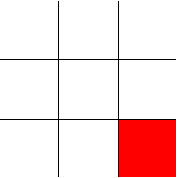
\includegraphics[width=0.33\textwidth]{con1}
	\captionof{figure}{Condition one}
\end{fixedpic}
\item Two fields occupied, one field empty. Here the condition occurs in the lowest row. Note how the first state occurs twice again, in the left and middle column.
\begin{fixedpic}
	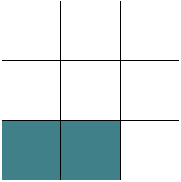
\includegraphics[width=0.33\textwidth]{con2}
	\captionof{figure}{Condition two}
\end{fixedpic}
\end{itemize}
The following three states are checked in the large field.
\begin{itemize}
\item One small field won, two small fields not yet determined. Here the condition occurs once in the top row. Here the first two states are no longer considered, a field is won a field is won.
\begin{fixedpic}
	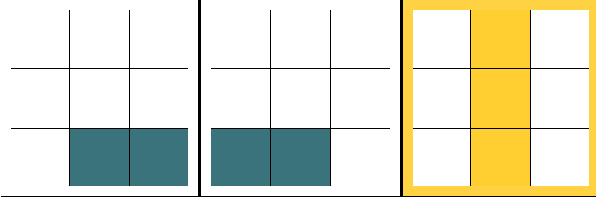
\includegraphics[width=0.33\textwidth]{con3}
	\captionof{figure}{Condition three}
\end{fixedpic}
\item Two small fields won, one small field not yet determined. Here is a visualization of this state.
\begin{fixedpic}
	\centering
	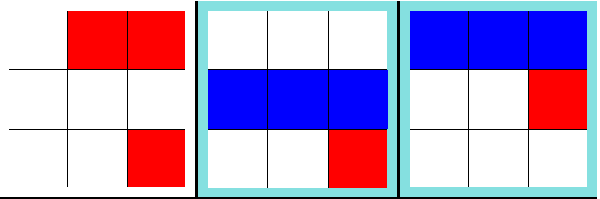
\includegraphics[width=0.6\textwidth]{con4}
	\captionof{figure}{Condition four}
\end{fixedpic}
\item Three small squares won. This also corresponds to a victory. Here the condition occurs in the right column.
\begin{fixedpic}
	\centering
	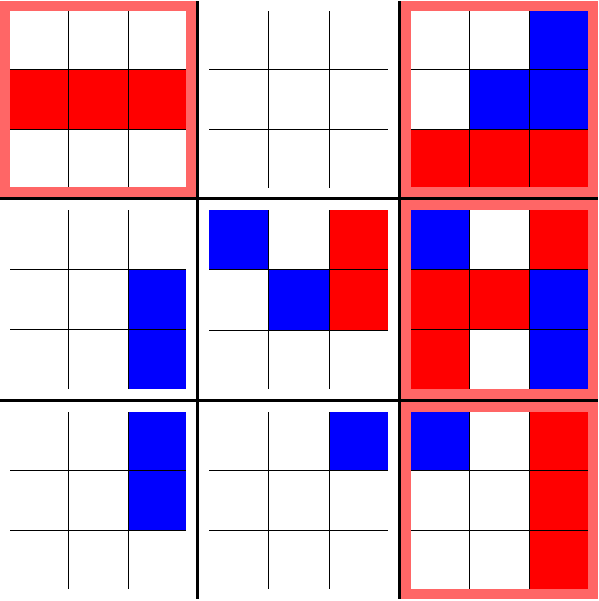
\includegraphics[width=0.6\textwidth]{con5}
	\captionof{figure}{Condition five}
\end{fixedpic}
\end{itemize}
Here I have drawn in all occurring states.
\begin{description}
\item[State one] Yellow
\item[State two] Green
\item[State three] Blue
\item[State four] Purple
\item[State five] Light blue
\end{description}
\begin{fixedpic}
	\centering
	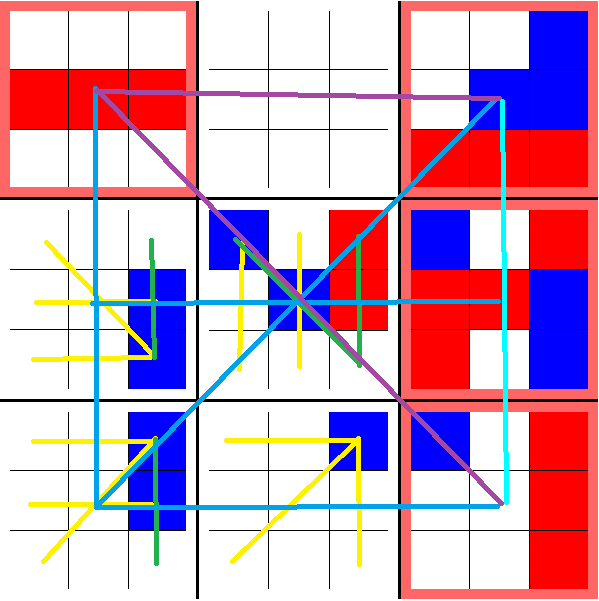
\includegraphics[width=0.6\textwidth]{allcons}
	\captionof{figure}{All Conditions}
\end{fixedpic}
The states are determined separately for both players. Now we take the difference of the states of the two players. Then we have a certain number for each state. Now we have to convert them into a meaningful number. This is where the DNA comes into play. The DNA is an object consisting of 5 fields. Each field stands for a factor by which the number of states is multiplied.
Let's do a sample calculation using the picture above. My DNA has the following Numbers.
\begin{description}
\item[Factor state one] 1
\item[Factor state two] 3
\item[Factor state three] 10
\item[Factor state four] 30
\item[Factor state five] 100
\end{description}\\
\begin{tabularx}{\textwidth}{|X|X|X|X|X|X|}
\hline
State & Occurrence red & Occurrence blue & Difference & Factor of DNA & Value \\\hline
1	& 0	& 11	& -11	& 1 	& -11 \\\hline
2	& 1	& 3 	& -2	& 3 	& -6 \\\hline
3	& 4	& 0 	& 4 	& 10	& 40 \\\hline
4	& 2	& 0 	& 2 	& 30	& 60 \\\hline
5	& 1	& 0 	& 1 	& 100	& 100 \\\hline
\multicolumn{5}{X|}{} & 183 \\\cline{6-6}
\end{tabularx}\\
The effective score in this case is 183, which is all the heuristic does. Based on this information, the Alpha Beta pruning decides which move to play.



\subsection{Self Learning}
To say it in easy terms, the self learning part learns how to estimate the game state in the most meaningful way. It learns which parameters are important in relation to the other parameters. In our case, the DNA  is responsible for that. The DNA dictates, which parameters are more important and it does that simply with a factor. The DNA is also the only thing which changes, while learning.

Let's take a look at how an algorithm is generated and how it gets better over time.
To start a new era, we need to set a few things up. An era can be compared to several generations of humans. 
The era contains all generations. In human generations, we have several individuals. In our case, we will call our individuals of the generation Organisms. We have to decide, how many Organisms per generation we want to create. But we have to keep in mind, the more Organisms we create, the longer the evolution will take. That's because every Organisms will play against every other Organisms twice. They play two times, to make sure every Organisms has once the possibility to start. The process of playing against each other is called selection. The Organisms get rewarded with 3 points when they win, and get 1 point when they end in a draw. When they loose, they won't get any points. The whole process of finding the best Organisms of a generation is actually very similar to a football cup.
%Formel 2*(n-1)
We also need to decide the search depth of the alpha beta pruning algorithm the organisms use, while playing against each other. The bigger the search depth, the longer it will take, because the computer has to calculate more scenarios. But the deeper we search, the more accurate results we will get. 
Now after we set up the amount of organisms and the search depth, we can start our new era. The first generation gets created (initialised) with random DNA. %in welchem bereich sind die Zufallszahlen?
That means the proportion of the different parameters vary vividly. We already know, the Organisms with the best random parameter configuration will perform the best. But we don't know yet exactly, which parameters are the most important ones. To find it out, which parameters are the best ones, we now let the organisms play against each other. In other words, we will start the selection. After all matches are finished, we can rank the organisms according to the point distribution system, which we used. The worse half of our first generation will die. And as it is in real evolution, mutation will take place.
The DNA of the better half of the ranking will mutate two times and form a new generation. The best Organism of the generation will survive and continue to live in the next generation.
%eventuell genäuere/bessere beschreibung
As described at the beginning, the mutation only affects the DNA. The DNA contains the factor for each parameter and each factor will be mutated by a value between 0.8 and 1.2. This results in an almost totally new set of Organisms, which are descenders of the previous generation. The selection starts again for this generation.
This cycle will continue as long as the creator of the era desires to. 

%
The era which is shown on our website contains 70 generations and each generation consists 16 Organisms.




\subsection{Implementation in Dart}

%For dynamic parts of a website, webbrowsers such as Google Chrome or Windows Explorer only understand a language called JavaScript. Because of that, our project, %which is mainly written in Dart, gets compiled (translated) to JavaScript. In that way, we can avoid the disadvantages JavaScript has.

\subsection{Website and User Interface}
In order that our project is accessible all over the world with different end devices ranging from Smartphones to Personal Computers running with different Operating Systems, we thought that it would be the most convenient solution to make a website. 


In general, the static part of the website is made with HTML (Hyper Text Markup Language) and CSS (Cascaded Style Sheets). HTML specifies the structure of a website.  CSS is then required to style everything. The dynamic part was already discussed in the previous subsection. 
Because CSS can be extremly time consuming, we made use of a CSS Framework called Materialize from Google, which provides cross browser compatible and responsible components such as navbars, buttons, dropdown-lists, cards, modals and many more. To make our website more appealing and fluid, we have used CSS animations. For this purpose, we used the website Animista, which provides ready-to-use CSS animations.

To deploy our website online, we also needed to have a host which offers a server and a domain. Because we already worked with tools of Google like the language Dart and the Materialize Framework, it wasn't far-fetched, that we decided to make use of a hosting provider which also belongs to Google. It's called Firebase. Firebase provides many options for developers such as Real Time Databases or Cloud Mesaging, but we only needed to use the hosting opportunity, which supports hosting static files like CSS, HTML.



Our website consists of two main parts. The first part is mainly designed for an easy game experience, where you can choose between three levels to play against the algorithm which include "easy", "medium" and "hard". Behind the easy level plays the best organism of the first generation. 
The medium level is played by the best organism of the 35th %evtl korrektur
generation and the hard level is the best organism of the whole era. The default search depth of the current game is three. Three is an experiential value, which is the best compromise between search duration and reliability of the algorithm.
The first part contains the rules of the game as well. 

Via a navbar link, it's possible to change to a more detailed and advanced view which we designed for people who are interested in what's going on behind the scenes. Its possible to see the whole era with all generations and organisms and it's evident, how the algorithm has evolved. It's also possible to generate a new era and calculate everything from scratch. As one plays against a desired Organism, it's also possible to adjust the search depth of the current game dynamically. It's observable, that it takes much longer for the algorithm to make a turn if the search depth is deeper. %evtl zeit erwähnen wie lange es geht

%evtl weglassen oder verbessern
Our Algorithm is separated from the part of the Web, that it is modular and reusable for any other applications like an app or something similar. In programming terms, things are separated with a thing called "Interface". Our Interface in dart is called the Player Interfacer. The Player Interface simply provides the information of our game state and is able to get input from the user interface on our website.
In HTML and CSS, we prepared a 9x9 grid, which we had to fill dynamically with the information of our Player Interface. When the algorithm made his turn, we also implementet a function that shows the player, where he has to play his next turn. 


\subsection{ Runtime } 

\subsubsection{ Device Restrictions}


\section{Progress Evaluation}


\section{Motivation}


\section{Review}
